\chapter{Pregled rezultata}
\label{chp:results}

Najmanje svojstvene vrijednosti trokuta numerički su izračunate metodom konačnih elemenata. Izvorni k\^{o}d programa za računanje tih vrijednosti vlastiti je rukopis napisan u programskom jeziku \href{https://freefem.org/}{\emph{FreeFem++}}, a inspiriran je primjerom za računanje svojstvenih vrijednosti i funkcija Laplaceovog operatora danim u~\cite{bib:Hecht19}. Metodu konačnih elemenata koristili su i Laugesen i Siudeja u~\cite{bib:Laugesen10}, stoga se takva metoda numeričkog računa svojstvenih vrijednosti Laplaceovog operatora u ovom radu smatra referentnim, klasičnim numeričkim računom (na njezinim rezultatima modeli su trenirani, a s njezinom brzinom i njom izračunatim vrijednostima uspoređuju se dobiveni modeli i njihova predviđanja).

\par

\section{Uspješnost modela}
\label{sec:models_success}

Uspješnost modela mjerila se dvama vrijednostima: korijenom srednje kvadratne greške (\emph{RMSE}) i srednjom postotnom apsolutnom greškom (\emph{MAPE}). Naime, budući da je najveća izmjerena svojstvena vrijednost više od $ \numprint{100} $ puta veća od najmanje, autor ovog rada smatra da \emph{RMSE} ne daje potpun uvid u uspješnost modela jer greška od $ {\pm \numprint{10}} $ nije jednako loša kod predviđanja stvarne vrijednosti $ \numprint{5000} $ i stvarne vrijednosti $ \numprint{50} $. No, svakako i \emph{MAPE} ne daje potpun uvid jer on ne pokazuje apsolutnu grešku. Vrijednosti \emph{RMSE} predviđanja modela na testnim skupovima podataka prikazani su u tablici~\ref{tab:models_rmse}, a \emph{MAPE} u tablici~\ref{tab:models_mape}.

\par%
\clearpage%
\newpage

\begin{table}[htb!]
    \centering
    \caption[Vrijednosti \emph{RMSE} predviđanja modela na testnim skupovima podataka]{Vrijednosti \emph{RMSE} predviđanja modela na testnim skupovima podataka. Polinom stupnja $ \numprint{4} $ označen je s $ P_{\numprint{4}} $, polinom stupnja $ \numprint{5} $ s $ P_{\numprint{5}} $, neuronska mreža s \emph{NN} i konvolucijska neuronska mreža s \emph{CNN}. Greške su posebno računate na $ \unit[\numprint{5}]{\%} $-tnim kvantilima ciljne varijable i na cijelom skupu. Svakom modelu crvenom bojom označena je najveća greška na kvantilima, a zelenom bojom najmanja.}
    \label{tab:models_rmse}
    \begin{tabular}{| r | c | r r r r |}
        \hline
        \multicolumn{2}{| c |}{$ \boldmath{\lambda}_{\numprint{1}} $} & \multicolumn{1}{c}{$ P_{\numprint{4}} $} & \multicolumn{1}{c}{$ P_{\numprint{5}} $} & \multicolumn{1}{c}{\emph{NN}} & \multicolumn{1}{c |}{\emph{CNN}} \\
        \hline
        $ \numprint{1} $. & $ \intervalco{\numprint{52.72}}{\numprint{55.41}} $ & $ \numprint{0.0329} $ & {\color{SeaGreen} $ \numprint{0.0229} $} & $ \numprint{1.6715} $ & {\color{SeaGreen} $ \numprint{0.9921} $} \\
        $ \numprint{2} $. & $ \intervalco{\numprint{55.41}}{\numprint{58.46}} $ & {\color{SeaGreen} $ \numprint{0.0317} $} & $ \numprint{0.0250} $ & {\color{SeaGreen} $ \numprint{0.4584} $} & $ \numprint{1.1883} $ \\
        $ \numprint{3} $. & $ \intervalco{\numprint{58.46}}{\numprint{62.06}} $ & $ \numprint{0.0405} $ & $ \numprint{0.0325} $ & $ \numprint{0.8638} $ & $ \numprint{1.1286} $ \\
        $ \numprint{4} $. & $ \intervalco{\numprint{62.06}}{\numprint{66.20}} $ & $ \numprint{0.0341} $ & $ \numprint{0.0322} $ & $ \numprint{1.0950} $ & $ \numprint{1.2021} $ \\
        $ \numprint{5} $. & $ \intervalco{\numprint{66.20}}{\numprint{71.01}} $ & $ \numprint{0.0459} $ & $ \numprint{0.0427} $ & $ \numprint{1.0259} $ & $ \numprint{1.4149} $ \\
        $ \numprint{6} $. & $ \intervalco{\numprint{71.01}}{\numprint{76.74}} $ & $ \numprint{0.0623} $ & $ \numprint{0.0536} $ & $ \numprint{0.5566} $ & $ \numprint{1.2677} $ \\
        $ \numprint{7} $. & $ \intervalco{\numprint{76.74}}{\numprint{83.51}} $ & $ \numprint{0.0671} $ & $ \numprint{0.0569} $ & $ \numprint{0.8077} $ & $ \numprint{1.4521} $ \\
        $ \numprint{8} $. & $ \intervalco{\numprint{83.51}}{\numprint{91.80}} $ & $ \numprint{0.0742} $ & $ \numprint{0.0801} $ & $ \numprint{0.6197} $ & $ \numprint{1.8222} $ \\
        $ \numprint{9} $. & $ \intervalco{\numprint{91.80}}{\numprint{102.00}} $ & $ \numprint{0.1042} $ & $ \numprint{0.1119} $ & $ \numprint{1.4973} $ & $ \numprint{2.0770} $ \\
        $ \numprint{10} $. & $ \intervalco{\numprint{102.00}}{\numprint{114.76}} $ & $ \numprint{0.1894} $ & $ \numprint{0.1794} $ & $ \numprint{0.5281} $ & $ \numprint{2.4864} $ \\
        $ \numprint{11} $. & $ \intervalco{\numprint{114.76}}{\numprint{130.69}} $ & $ \numprint{0.2551} $ & $ \numprint{0.2296} $ & $ \numprint{0.7137} $ & $ \numprint{3.2092} $ \\
        $ \numprint{12} $. & $ \intervalco{\numprint{130.69}}{\numprint{152.54}} $ & $ \numprint{0.6292} $ & $ \numprint{0.6233} $ & $ \numprint{0.8131} $ & $ \numprint{4.0720} $ \\
        $ \numprint{13} $. & $ \intervalco{\numprint{152.54}}{\numprint{181.99}} $ & $ \numprint{1.0101} $ & $ \numprint{1.0006} $ & $ \numprint{1.1977} $ & $ \numprint{4.7786} $ \\
        $ \numprint{14} $. & $ \intervalco{\numprint{181.99}}{\numprint{221.86}} $ & $ \numprint{1.4744} $ & $ \numprint{1.4844} $ & $ \numprint{1.6966} $ & $ \numprint{5.4182} $ \\
        $ \numprint{15} $. & $ \intervalco{\numprint{221.86}}{\numprint{282.86}} $ & $ \numprint{1.5497} $ & $ \numprint{1.4995} $ & $ \numprint{1.6110} $ & $ \numprint{6.4026} $ \\
        $ \numprint{16} $. & $ \intervalco{\numprint{282.86}}{\numprint{381.22}} $ & $ \numprint{4.1479} $ & $ \numprint{3.9177} $ & $ \numprint{3.4231} $ & $ \numprint{8.8674} $ \\
        $ \numprint{17} $. & $ \intervalco{\numprint{381.22}}{\numprint{541.76}} $ & $ \numprint{5.5007} $ & $ \numprint{4.6252} $ & $ \numprint{3.3480} $ & $ \numprint{13.4791} $ \\
        $ \numprint{18} $. & $ \intervalco{\numprint{541.76}}{\numprint{861.51}} $ & $ \numprint{6.0323} $ & $ \numprint{6.9183} $ & $ \numprint{5.5581} $ & $ \numprint{18.2880} $ \\
        $ \numprint{19} $. & $ \intervalco{\numprint{861.51}}{\numprint{1714.84}} $ & $ \numprint{20.8065} $ & $ \numprint{20.7103} $ & $ \numprint{10.6677} $ & $ \numprint{22.9396} $ \\
        $ \numprint{20} $. & $ \intervalcc{\numprint{1714.84}}{\numprint{5942.29}} $ & {\color{FireBrick} $ \numprint{161.7162} $} & {\color{FireBrick} $ \numprint{130.3451} $} & {\color{FireBrick} $ \numprint{32.1044} $} & {\color{FireBrick} $ \numprint{79.7745} $} \\
        \hline
        \multicolumn{2}{| c |}{Ukupno} & $ \numprint{36.5206} $ & $ \numprint{29.5883} $ & $ \numprint{7.7983} $ & $ \numprint{19.5316} $ \\
        \hline
    \end{tabular}
\end{table}

\par

Svi modeli najveći \emph{RMSE} postižu na gornjih $ \unit[\numprint{5}]{\%} $ vrijednosti ciljne varijable, a najmanji na prvih ili drugih najmanjih $ \unit[\numprint{5}]{\%} $. Polinomni modeli na najviše kvantila postižu \emph{RMSE} strogo manji od $ \numprint{1} $, a čak na $ \numprint{8} $ kvantila postižu \emph{RMSE} strogo manji i od $ \numprint{0.1} $. S druge strane, najmanji kvantilni \emph{RMSE} koji neuronska mreža postiže veći je od $ \numprint{0.4} $, dok kod konvolucijske neuronske mreže on iznosi gotovo $ \numprint{1} $. Ipak, neuronska mreža, uspoređujući \emph{RMSE}, osjetno prednjači u posljednja dva kvantila, kao i na cijelom testnom skupu podataka. Polinomni modeli, iako točniji na nižim kvantilima, u posljednjem su kvantilu i na cijelom testnom skupu vidno najlošiji po vrijednostima \emph{RMSE}.

\par%
\clearpage%
\newpage

\begin{table}[htb!]
    \centering
    \caption[Vrijednosti \emph{MAPE} predviđanja modela na testnim skupovima podataka]{Vrijednosti \emph{MAPE} predviđanja modela na testnim skupovima podataka. Polinom stupnja $ \numprint{4} $ označen je s $ P_{\numprint{4}} $, polinom stupnja $ \numprint{5} $ s $ P_{\numprint{5}} $, neuronska mreža s \emph{NN} i konvolucijska neuronska mreža s \emph{CNN}. Greške su posebno računate na $ \unit[\numprint{5}]{\%} $-tnim kvantilima ciljne varijable i na cijelom skupu. Svakom modelu crvenom bojom označena je najveća greška na kvantilima, a zelenom bojom najmanja.}
    \label{tab:models_mape}
    \begin{tabular}{| r | c | r r r r |}
        \hline
        \multicolumn{2}{| c |}{$ \lambda_{\numprint{1}} $} & \multicolumn{1}{c}{$ P_{\numprint{4}} $} & \multicolumn{1}{c}{$ P_{\numprint{5}} $} & \multicolumn{1}{c}{\emph{NN}} & \multicolumn{1}{c |}{\emph{CNN}} \\
        \hline
        $ \numprint{1} $. & $ \intervalco{\numprint{52.72}}{\numprint{55.41}} $ & $ \unit[\numprint{0.0487}]{\%} $ & {\color{SeaGreen} $ \unit[\numprint{0.0314}]{\%} $} & {\color{FireBrick} $ \unit[\numprint{2.9542}]{\%} $} & $ \unit[\numprint{1.5331}]{\%} $ \\
        $ \numprint{2} $. & $ \intervalco{\numprint{55.41}}{\numprint{58.46}} $ & $ \unit[\numprint{0.0454}]{\%} $ & $ \unit[\numprint{0.0373}]{\%} $ & $ \unit[\numprint{0.6750}]{\%} $ & $ \unit[\numprint{1.6503}]{\%} $ \\
        $ \numprint{3} $. & $ \intervalco{\numprint{58.46}}{\numprint{62.06}} $ & $ \unit[\numprint{0.0575}]{\%} $ & $ \unit[\numprint{0.0445}]{\%} $ & $ \unit[\numprint{1.2708}]{\%} $ & $ \unit[\numprint{1.5000}]{\%} $ \\
        $ \numprint{4} $. & $ \intervalco{\numprint{62.06}}{\numprint{66.20}} $ & {\color{SeaGreen} $ \unit[\numprint{0.0425}]{\%} $} & $ \unit[\numprint{0.0380}]{\%} $ & $ \unit[\numprint{1.4100}]{\%} $ & $ \unit[\numprint{1.4998}]{\%} $ \\
        $ \numprint{5} $. & $ \intervalco{\numprint{66.20}}{\numprint{71.01}} $ & $ \unit[\numprint{0.0508}]{\%} $ & $ \unit[\numprint{0.0500}]{\%} $ & $ \unit[\numprint{1.3413}]{\%} $ & $ \unit[\numprint{1.6866}]{\%} $ \\
        $ \numprint{6} $. & $ \intervalco{\numprint{71.01}}{\numprint{76.74}} $ & $ \unit[\numprint{0.0673}]{\%} $ & $ \unit[\numprint{0.0586}]{\%} $ & $ \unit[\numprint{0.5972}]{\%} $ & $ \unit[\numprint{1.4042}]{\%} $ \\
        $ \numprint{7} $. & $ \intervalco{\numprint{76.74}}{\numprint{83.51}} $ & $ \unit[\numprint{0.0624}]{\%} $ & $ \unit[\numprint{0.0512}]{\%} $ & $ \unit[\numprint{0.8469}]{\%} $ & $ \unit[\numprint{1.4894}]{\%} $ \\
        $ \numprint{8} $. & $ \intervalco{\numprint{83.51}}{\numprint{91.80}} $ & $ \unit[\numprint{0.0674}]{\%} $ & $ \unit[\numprint{0.0745}]{\%} $ & $ \unit[\numprint{0.6177}]{\%} $ & $ \unit[\numprint{1.5475}]{\%} $ \\
        $ \numprint{9} $. & $ \intervalco{\numprint{91.80}}{\numprint{102.00}} $ & $ \unit[\numprint{0.0801}]{\%} $ & $ \unit[\numprint{0.0875}]{\%} $ & $ \unit[\numprint{1.4076}]{\%} $ & $ \unit[\numprint{1.6737}]{\%} $ \\
        $ \numprint{10} $. & $ \intervalco{\numprint{102.00}}{\numprint{114.76}} $ & $ \unit[\numprint{0.1338}]{\%} $ & $ \unit[\numprint{0.1349}]{\%} $ & {\color{SeaGreen} $ \unit[\numprint{0.3902}]{\%} $} & $ \unit[\numprint{1.8423}]{\%} $ \\
        $ \numprint{11} $. & $ \intervalco{\numprint{114.76}}{\numprint{130.69}} $ & $ \unit[\numprint{0.1589}]{\%} $ & $ \unit[\numprint{0.1465}]{\%} $ & $ \unit[\numprint{0.4826}]{\%} $ & $ \unit[\numprint{2.1209}]{\%} $ \\
        $ \numprint{12} $. & $ \intervalco{\numprint{130.69}}{\numprint{152.54}} $ & $ \unit[\numprint{0.3794}]{\%} $ & $ \unit[\numprint{0.3659}]{\%} $ & $ \unit[\numprint{0.4706}]{\%} $ & {\color{FireBrick} $ \unit[\numprint{2.4063}]{\%} $} \\
        $ \numprint{13} $. & $ \intervalco{\numprint{152.54}}{\numprint{181.99}} $ & $ \unit[\numprint{0.5090}]{\%} $ & $ \unit[\numprint{0.5031}]{\%} $ & $ \unit[\numprint{0.5713}]{\%} $ & $ \unit[\numprint{2.3786}]{\%} $ \\
        $ \numprint{14} $. & $ \intervalco{\numprint{181.99}}{\numprint{221.86}} $ & $ \unit[\numprint{0.5008}]{\%} $ & $ \unit[\numprint{0.5048}]{\%} $ & $ \unit[\numprint{0.6333}]{\%} $ & $ \unit[\numprint{2.1816}]{\%} $ \\
        $ \numprint{15} $. & $ \intervalco{\numprint{221.86}}{\numprint{282.86}} $ & $ \unit[\numprint{0.4969}]{\%} $ & $ \unit[\numprint{0.4712}]{\%} $ & $ \unit[\numprint{0.4650}]{\%} $ & $ \unit[\numprint{2.0293}]{\%} $ \\
        $ \numprint{16} $. & $ \intervalco{\numprint{282.86}}{\numprint{381.22}} $ & $ \unit[\numprint{1.0267}]{\%} $ & $ \unit[\numprint{0.9752}]{\%} $ & $ \unit[\numprint{0.7985}]{\%} $ & $ \unit[\numprint{2.1396}]{\%} $ \\
        $ \numprint{17} $. & $ \intervalco{\numprint{381.22}}{\numprint{541.76}} $ & $ \unit[\numprint{0.9959}]{\%} $ & $ \unit[\numprint{0.8211}]{\%} $ & $ \unit[\numprint{0.5761}]{\%} $ & $ \unit[\numprint{2.4052}]{\%} $ \\
        $ \numprint{18} $. & $ \intervalco{\numprint{541.76}}{\numprint{861.51}} $ & $ \unit[\numprint{0.7094}]{\%} $ & $ \unit[\numprint{0.8147}]{\%} $ & $ \unit[\numprint{0.6398}]{\%} $ & $ \unit[\numprint{2.1040}]{\%} $ \\
        $ \numprint{19} $. & $ \intervalco{\numprint{861.51}}{\numprint{1714.84}} $ & $ \unit[\numprint{1.0326}]{\%} $ & $ \unit[\numprint{1.3081}]{\%} $ & $ \unit[\numprint{0.6738}]{\%} $ & {\color{SeaGreen} $ \unit[\numprint{1.3769}]{\%} $} \\
        $ \numprint{20} $. & $ \intervalcc{\numprint{1714.84}}{\numprint{5942.29}} $ & {\color{FireBrick} $ \unit[\numprint{3.4702}]{\%} $} & {\color{FireBrick} $ \unit[\numprint{2.5835}]{\%} $} & $ \unit[\numprint{0.7544}]{\%} $ & $ \unit[\numprint{1.7879}]{\%} $ \\
        \hline
        \multicolumn{2}{| c |}{Ukupno} & $ \unit[\numprint{0.4968}]{\%} $ & $ \unit[\numprint{0.4551}]{\%} $ & $ \unit[\numprint{0.8788}]{\%} $ & $ \unit[\numprint{1.8379}]{\%} $ \\
        \hline
    \end{tabular}
\end{table}

\par

Zanimljiva je pojava da neuronska mreža najveću vrijednost \emph{MAPE} postiže na najdonjem kvantilu ciljne varijable, dok, na primjer, na tom kvantilu polinom stupnja $ \numprint{5} $ postiže najmanju vrijednost \emph{MAPE}. Štoviše, vrijednost \emph{MAPE} neuronske mreže na najdonjem kvantilu druga je najveća vrijednost \emph{MAPE} svih modela, dok je vrijednost \emph{MAPE} polinoma stupnja $ \numprint{5} $ na tom kvantilu najmanja među svim modelima. I kod vrijednosti \emph{MAPE} polinomna rješenja prednjače po broju kvantila s najnižim greškama, ali, za razliku od \emph{RMSE}, po vrijednosti \emph{MAPE} od neuronske mreže i od konvolucijske neuronske mreže bolji su i na cijelom testnom skupu podataka. Promatrajući \emph{MAPE}, najlošije rezultate postiže konvolucijska neuronska mreža---na najviše kvantila postiže vrijednost \emph{MAPE} veću od $ \unit[\numprint{2}]{\%} $, ni na jednom kvantilu ne postiže vrijednost \emph{MAPE} strogo manju od $ \unit[\numprint{1}]{\%} $ i na cijelom testnom skupu podataka više je nego dvostruko lošija od ostalih modela. Ipak, najlošija vrijednost \emph{MAPE} konvolucijske neuronske mreže najmanja je najlošija vrijednost \emph{MAPE} svih modela.

\par

Vizualni prikazi predviđanja modela na svim vrijednostima dani su na slikama~\ref{fig:polynomial_predictions} i \ref{fig:networks_predictions}, a na donjih $ \unit[\numprint{90}]{\%} $ vrijednosti na slikama~\ref{fig:polynomial_predictions_90_percent} i \ref{fig:networks_predictions_90_percent}---potonje dvije slike posebno su izrađene zbog nesrazmjernih veličina kvantila (donjih $ \unit[\numprint{90}]{\%} $ u intervalu je širine manje od $ \numprint{1000} $, a gornjih $ \unit[\numprint{10}]{\%} $ u intervalu širem od $ \numprint{5000} $). Na tim je slikama za svaku vrijednost ciljne varijable $ \lambda_{\numprint{1}} $ u testnom skupu podataka prikazana predviđena vrijednost $ \text{\texttt{predicted value}} $ kao točka s koordinatama $ \left( \lambda_{1} , \text{\texttt{predicted value}} \right) $. Osim predviđanja, naznačena je linija identitete kao poželjni položaji predviđanja (točke predviđanja na tom pravcu predstavljale bi savršeno predviđanje s greškom $ \numprint{0} $). Kao što se iz tablice~\ref{tab:models_rmse} može i naslutiti, vizualno \emph{najstabilniji} je u predviđanju većih vrijednosti model neuronske mreže. Na slikama se, također, jasno vidi kako modeli (pogotovo polinomi) na većim vrijednostima počinju sve više griješiti, što sugeriraju tablice~\ref{tab:models_rmse} i \ref{tab:models_mape}. S druge strane, na manjim vrijednostima svi su modeli precizniji, a, kao što se iz tablica~\ref{tab:models_rmse} i \ref{tab:models_mape} već može naslutiti, polinomni modeli vrlo precizno predviđaju male vrijednosti ciljne varijable.

\par%
\clearpage%
\newpage

\begin{figure}[htb!]
    \centering
    \begin{subfigure}{57mm}
        \centering
        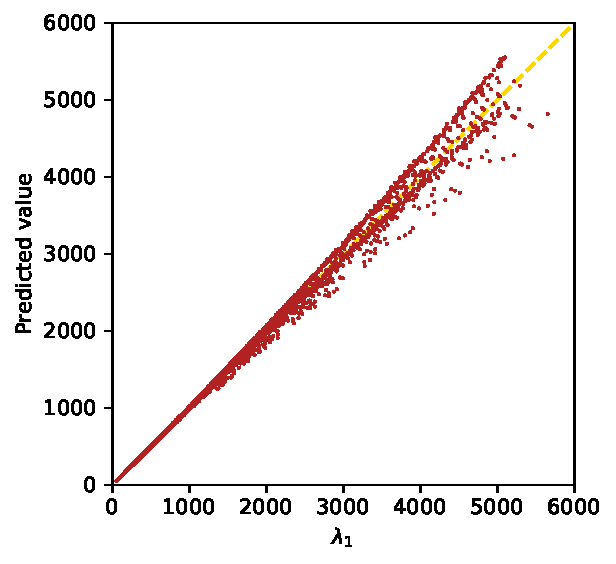
\includegraphics[width = 52mm]{figures/polynomial_4_prediction.pdf}
        \caption{Predviđanja \ensuremath{P_{\numprint{4}}}}
        \label{fig:polynomial_4_prediction}
    \end{subfigure}
    \begin{subfigure}{57mm}
        \centering
        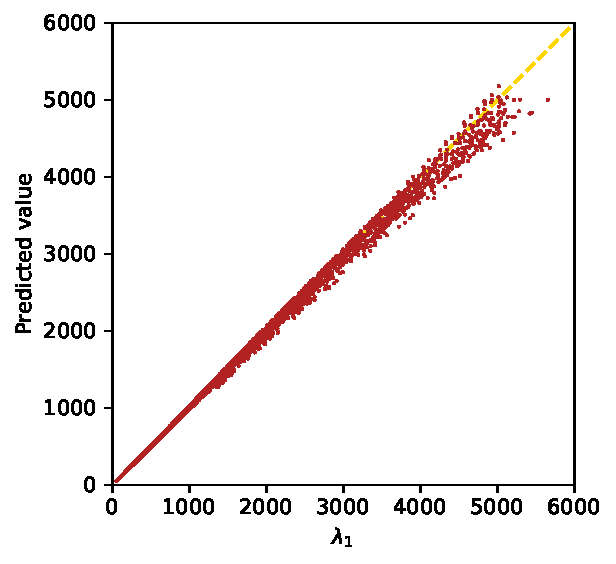
\includegraphics[width = 52mm]{figures/polynomial_5_prediction.pdf}
        \caption{Predviđanja \ensuremath{P_{\numprint{5}}}}
        \label{fig:polynomial_5_prediction}
    \end{subfigure}
    \caption[Predviđanja polinoma]{Predviđanja polinoma. Polinom stupnja $ \numprint{4} $ označen je s $ P_{\numprint{4}} $ i polinom stupnja $ \numprint{5} $ s $ P_{\numprint{5}} $.}
    \label{fig:polynomial_predictions}
\end{figure}

\par

\begin{figure}[htb!]
    \centering
    \begin{subfigure}{57mm}
        \centering
        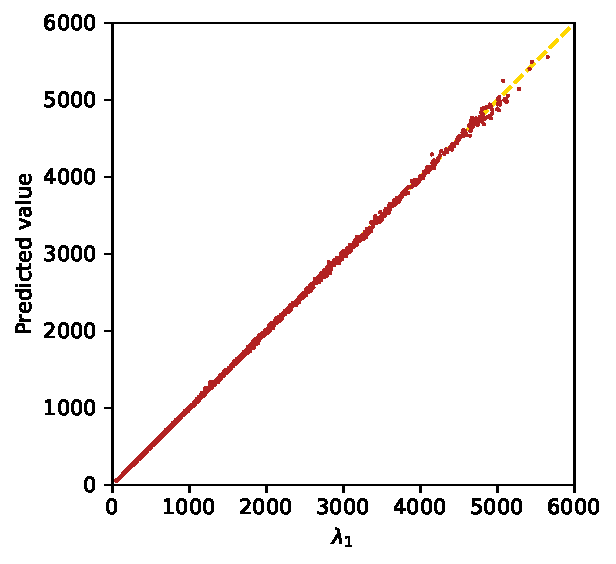
\includegraphics[width = 52mm]{figures/neural_network_prediction.pdf}
        \caption{Predviđanja \emph{NN}}
        \label{fig:neural_network_prediction}
    \end{subfigure}
    \begin{subfigure}{57mm}
        \centering
        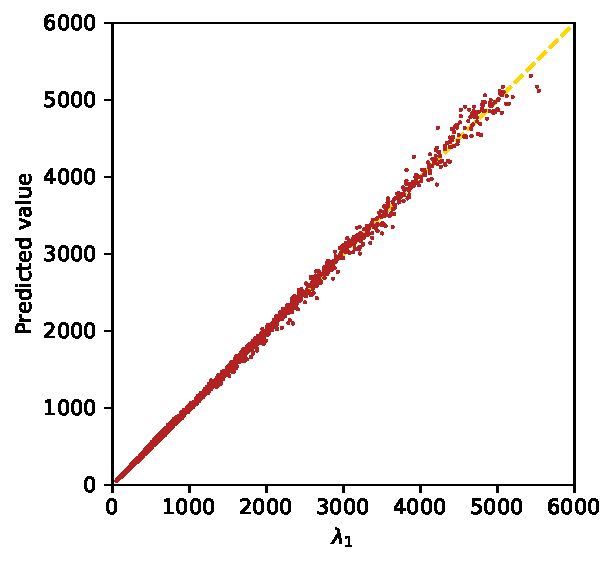
\includegraphics[width = 52mm]{figures/convolutional_neural_network_prediction.pdf}
        \caption{Predviđanja \emph{CNN}}
        \label{fig:convolutional_neural_network_prediction}
    \end{subfigure}
    \caption[Predviđanja neuronske mreže i konvolucijske neuronske mreže]{Predviđanja neuronske mreže i konvolucijske neuronske mreže. Neuronska mreža označena je s \emph{NN} i konvolucijska neuronska mreža s \emph{CNN}.}
    \label{fig:networks_predictions}
\end{figure}

\par%
\clearpage%
\newpage

\begin{figure}[htb!]
    \centering
    \begin{subfigure}{55.5mm}
        \centering
        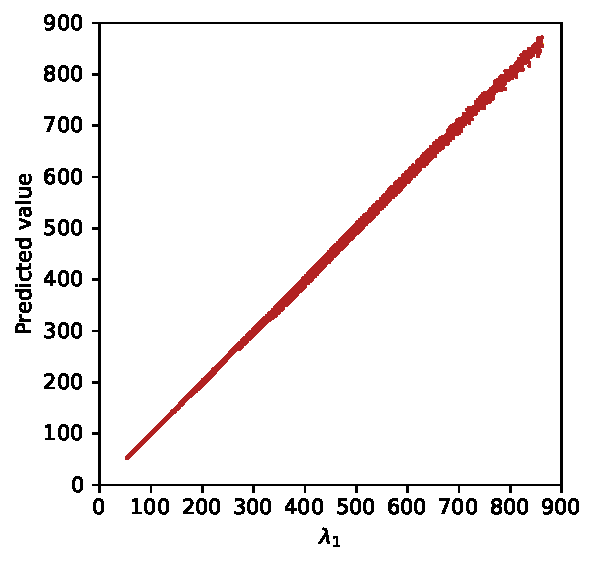
\includegraphics[width = 50.5mm]{figures/polynomial_4_prediction_90_percent.pdf}
        \caption{Predviđanja \ensuremath{P_{\numprint{4}}}}
        \label{fig:polynomial_4_prediction_90_percent}
    \end{subfigure}
    \begin{subfigure}{55.5mm}
        \centering
        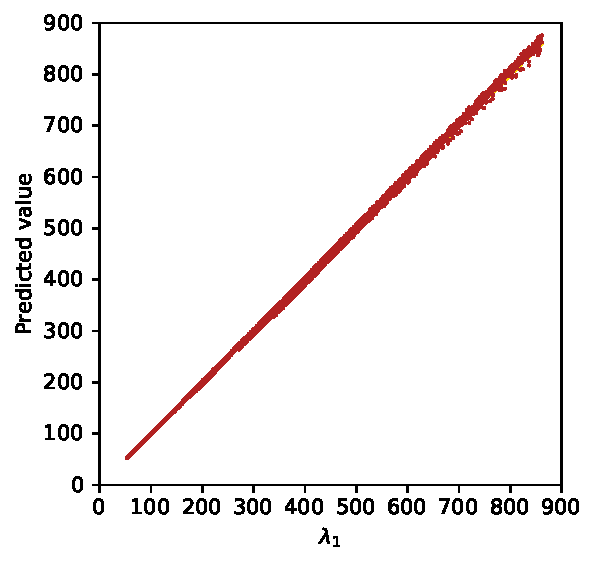
\includegraphics[width = 50.5mm]{figures/polynomial_5_prediction_90_percent.pdf}
        \caption{Predviđanja \ensuremath{P_{\numprint{5}}}}
        \label{fig:polynomial_5_prediction_90_percent}
    \end{subfigure}
    \caption[Predviđanja polinoma na donjih \ensuremath{\unit[\numprint{90}]{\%}} vrijednosti]{Predviđanja polinoma na donjih \ensuremath{\unit[\numprint{90}]{\%}} vrijednosti. Polinom stupnja $ \numprint{4} $ označen je s $ P_{\numprint{4}} $ i polinom stupnja $ \numprint{5} $ s $ P_{\numprint{5}} $.}
    \label{fig:polynomial_predictions_90_percent}
\end{figure}

\par

\begin{figure}[htb!]
    \centering
    \begin{subfigure}{55.5mm}
        \centering
        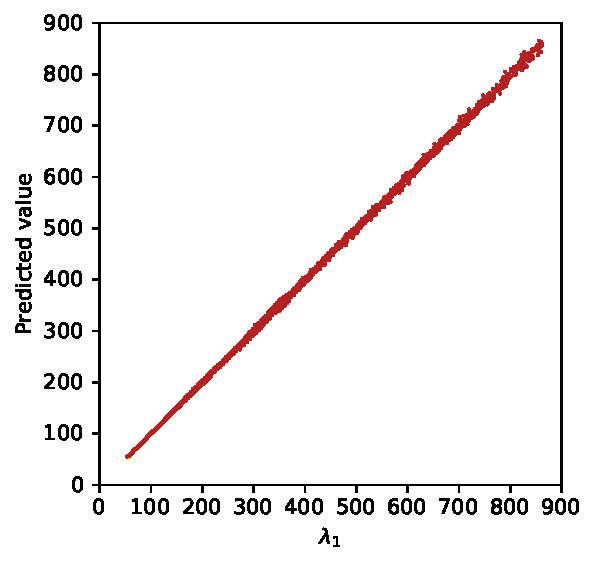
\includegraphics[width = 50.5mm]{figures/neural_network_prediction_90_percent.pdf}
        \caption{Predviđanja \emph{NN}}
        \label{fig:neural_network_prediction_90_percent}
    \end{subfigure}
    \begin{subfigure}{55.5mm}
        \centering
        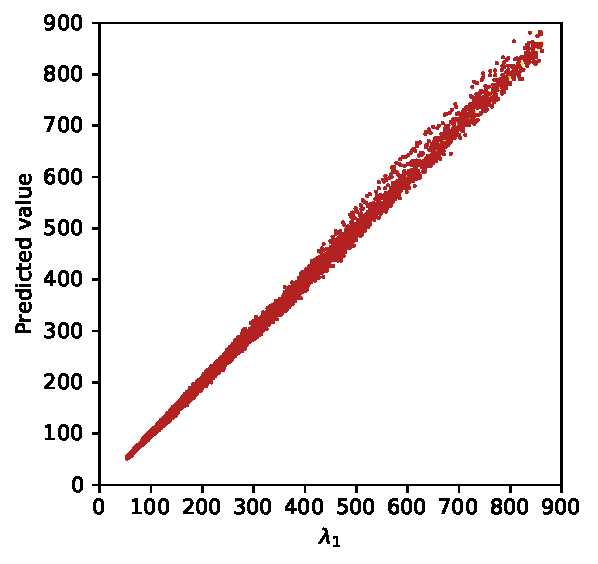
\includegraphics[width = 50.5mm]{figures/convolutional_neural_network_prediction_90_percent.pdf}
        \caption{Predviđanja \emph{CNN}}
        \label{fig:convolutional_neural_network_prediction_90_percent}
    \end{subfigure}
    \caption[Predviđanja neuronske mreže i konvolucijske neuronske mreže na donjih \ensuremath{\unit[\numprint{90}]{\%}} vrijednosti]{Predviđanja neuronske mreže i konvolucijske neuronske mreže na donjih \ensuremath{\unit[\numprint{90}]{\%}} vrijednosti. Neuronska mreža označena je s \emph{NN} i konvolucijska neuronska mreža s \emph{CNN}.}
    \label{fig:networks_predictions_90_percent}
\end{figure}

\par%
\clearpage%
\newpage

\section{Brzine modela}
\label{sec:models_time_consumption}

Za usporedbu brzina modela, modeli su provedeni na kompletnom skupu podataka od $ \numprint{1129741} $ trokuta iako su među njima i trokuti iz testnih i validacijskih skupova. Međutim, za računanje brzine modela točnosti tih predviđanja nisu se proučavale, a skup od više od $ \numprint{1000000} $ trokuta predstavljao je dovoljno velik skup za objektivno mjerenje vremena (više pokretanja iste metode vremenski je vrlo malo variralo). Metode su pokretane na osobnom prijenosnom računalu autora kao jedini korisnikovi pokrenuti procesi nakon pokretanja operacijskog sustava, a svaka metoda pokrenuta je $ \numprint{3} $ puta i kao konačno vrijeme uzeta je aritmetička sredina triju izmjerenih vremena.

\par

Referentno računalo opremljeno je procesorom \emph{\href{https://www.intel.co.uk/}{Intel{\textregistered}} Core{\texttrademark} i$ \numprint{5} $-$ \numprint{7200} $U $ \SI{2.5}{\giga \hertz} $} s \emph{Turbo Boost} ubrzanjem do $ \SI{3.1}{\giga \hertz} $, s $ \SI{8}{\giga \byte} $ \emph{DDR$ \numprint{4} $} radne memorije i s grafičkom karticom \emph{\href{https://www.nvidia.com/}{NVIDIA{\textregistered}} GeForce{\textregistered} GTX $ \numprint{950} $M} s $ \SI{2}{\giga \byte} $ \emph{VRAM}-a. Korišteni operacijski sustav je \href{https://www.linux.org/}{\emph{Linux}} distribucija \emph{\href{https://lubuntu.net/}{Lubuntu} $ \numprint{18} $.$ \numprint{04} $}, prevoditelj programskog jezika \href{https://en.cppreference.com/w/c/header}{\emph{C}} je \emph{\href{https://gcc.gnu.org/}{GCC} $ \numprint{7} $.$ \numprint{4} $.$ \numprint{0} $} i inačica programskog jezika \href{https://docs.python.org/3/}{\emph{Python}} je $ \numprint{3} $.$ \numprint{6} $.$ \numprint{9} $. Inačica paketa \href{https://numpy.org/}{\emph{NumPy}} je $ \numprint{1} $.$ \numprint{17} $.$ \numprint{4} $, paketa \href{https://pandas.pydata.org/}{\emph{Pandas}} $ \numprint{0} $.$ \numprint{25} $.$ \numprint{3} $, paketa \href{https://scikit-learn.org/stable/}{\emph{Scikit-learn}} $ \numprint{0} $.$ \numprint{22} $, paketa \href{https://www.tensorflow.org/}{\emph{TensorFlow}} $ \numprint{1} $.$ \numprint{14} $.$ \numprint{0} $ i paketa \href{https://keras.io/}{\emph{Keras}} $ \numprint{2} $.$ \numprint{3} $.$ \numprint{1} $. Inačica platforme \href{https://developer.nvidia.com/cuda-zone}{\emph{CUDA}} je $ \numprint{10} $.$ \numprint{2} $.$ \numprint{89} $. Interpreter programskog jezika \href{https://freefem.org/}{\emph{FreeFem++}} inačice je $ \numprint{4} $.$ \numprint{400003} $.

\par

Rezultati mjerenja vremena prikazani su u tablici~\ref{tab:computation_times}. Brzina modela konvolucijske neuronske mreže nije izračunata zbog nedostatka resursa, ali i zbog nedovoljno optimiziranog algoritma generiranja vizualizacija trokuta. Naime, na platformi \href{https://colab.research.google.com/}{\emph{Google Colab}} generiranje vizualizacija trokuta, koje bi se smatralo pretprocesiranjem za model konvolucijske neuronske mreže (osnovnim ulaznim podatcima svih modela smatraju se koordinate vrhova trokuta), na $ \numprint{100000} $ trokuta trajalo je dulje od, na primjer, računanja svojstvenih vrijednosti metodom konačnih elemenata na referentnom računalu, koje je slabijih specifikacija.

\par%
\clearpage%
\newpage

\begin{table}[htb!]
    \centering
    \caption[Usporedba vremena metoda računanja]{Usporedba vremena metoda računanja. \emph{FEM} je numerički račun metodom konačnih elemenata, \emph{deskripcija} je računanje duljina stranica i veličina vanjskih kutova, \emph{uređenje} je poredanje duljina stranica u padajući poredak i veličina vanjskih kutova u rastući, \emph{karakterizacija} je računanje koordinata karakteristične točke (\seetxt~propoziciju~\ref{prop:triangle_characteristic_bijective}) iz rezultata \emph{deskripcije}, a \emph{SVD} je računanje singularnih vrijednosti duljina stranica i vanjskih kutova iz rezultata \emph{deskripcije}.}
    \label{tab:computation_times}
    \begin{tabular}{| c | l | r  r |}
        \hline
        \multicolumn{1}{| c |}{Područje} & \multicolumn{1}{c |}{Opis} & \multicolumn{1}{c}{Apsolutno vrijeme} & \multicolumn{1}{c |}{Relativno vrijeme} \\
        \hline
        \multirow{1}{*}{Numerički račun} & \emph{FEM} & $ \SI{948.754328}{\second} $ & $ \numprint{1.000000} $ \\
        \hline
        \multirow{4}{*}{Pretprocesiranje} & Deskripcija & $ \SI{0.180276}{\second} $ & $ \numprint{0.000190} $ \\
         & Uređenje & $ \SI{0.080183}{\second} $ & $ \numprint{0.000085} $ \\
         & Karakterizacija & $ \SI{0.054539}{\second} $ & $ \numprint{0.000057} $ \\
         & \emph{SVD} & $ \SI{4.821884}{\second} $ & $ \numprint{0.005082} $ \\
        \hline
        \multirow{3}{*}{Predviđanje} & Polinom stupnja $ \numprint{4} $ & $ \SI{0.433055}{\second} $ & $ \numprint{0.000456} $ \\
         & Polinom stupnja $ \numprint{5} $ & $ \SI{0.690426}{\second} $ & $ \numprint{0.000728} $ \\
         & Neuronska mreža & $ \SI{1.014543}{\second} $ & $ \numprint{0.001069} $ \\
        \hline
    \end{tabular}
\end{table}

\par

Iz tablice~\ref{tab:computation_times} možemo zaključiti da je, i ako ubrojimo odgovarajuće pretprocesiranje, polinom stupnja $ \numprint{4} $ od klasičnog numeričkog računa brži čak više od $ \numprint{1422} $ puta, a polinom stupnja $ \numprint{5} $ brži je više od $ \numprint{1025} $ puta. Neuronska mreža brža je više od $ \numprint{155} $ puta, pri čemu skoro $ \unit[80]{\%} $ vremena za model neuronske mreže zauzima \emph{SVD}. Ako se \emph{SVD} trokuta može vremenski optimizirati, takvo bi poboljšanje moglo bitno ubrzati ovaj model.

\par

\section{Minimizacija najmanje svojstvene vrijednosti Laplaceovog operatora}
\label{sec:minimal_Laplace_eigenvalue_minimisation}

Osim po globalnoj uspješnosti i brzini, modeli su testirani i u simuliranom primjeru stvarne primjene. U tu je svrhu uzet problem minimizacije najmanje svojstvene vrijednosti na trokutima fiksnog opsega. Najmanja svojstvena vrijednost Laplaceovog operatora morala bi se postizati na jednakostraničnom trokutu, što proizlazi iz nejednakosti vezanih uz površinu skupa koje je Siudeja naveo u~\cite{bib:Siudeja08} i Heronove formule za površinu trokuta. Laugesen i Siudeja u~\cite{bib:Laugesen10} također su iskazali da, osim među trokutima fiksnog opsega ili fiksne površine, jednakostranični trokut najmanju svojstvenu vrijednost minimizira i među trokutima fiksnog dijametra, što se može i naslutiti iz slike~\ref{fig:triangles_eigenvalues}.

\par

Proučavana su dva problema minimizacije. Jedan je u $ \numprint{6} $-dimenzionalnom prostoru, to jest, pronalazak (nekih) vrijednosti $ x_{\numprint{1}} , y_{\numprint{1}} , x_{\numprint{2}} , y_{\numprint{2}} , x_{\numprint{3}} , y_{\numprint{3}} \in \reals $ takvih da je trokut čiji su vrhovi dani koordinatama $ \left( x_{\numprint{1}} , y_{\numprint{1}} \right) , \left( x_{\numprint{2}} , y_{\numprint{2}} \right) , \left( x_{\numprint{3}} , y_{\numprint{3}} \right) \in \reals^{\numprint{2}} $ u standardnoj bazi opsega $ \numprint{3} $ i da među takvim trokutima on postiže najnižu najmanju svojstvenu vrijednost Laplaceovog operatora---teorem~\ref{thm:Laplacian_eigenvalue_similar_domains} odnosno korolar~\ref{cor:spectrum_similar_domains} pokazuju da takvih (jednakostraničnih) trokuta ima neprebrojivo beskonačno mnogo, ali su svi oni jednaki do na izometrične transformacije. Drugi je problem u $ \numprint{1} $-dimenzionalnom prostoru, to jest, pronaći vrijednost $ \varphi \in \intervaloo{\numprint{0}}{\pi} $ takvu da trokut čiji su vrhovi dani koordinatama $ \left( \frac{\numprint{1}}{\numprint{2}} , \numprint{0} \right) , \left( \cos \varphi , \frac{\sqrt{\numprint{3}}}{\numprint{2}} \sin \varphi \right) , \left( {- \frac{\numprint{1}}{\numprint{2}}} , \numprint{0} \right) \in \reals^{\numprint{2}} $ u standardnoj bazi među takvim trokutima postiže najnižu najmanju svojstvenu vrijednost---ovdje je rješenje jedinstveno i iznosi $ \varphi = \frac{\pi}{\numprint{2}} $ (uz uvjet $ \varphi \in \intervaloo{{- \pi}}{\pi} \setminus \left\{ \numprint{0} \right\} $ rješenja bi bila $ \varphi = {\pm \frac{\pi}{\numprint{2}}} $, a za $ \varphi \in \reals \setminus \left\{ k \pi \in \reals : k \in \integers \right\} $ sva su rješenja od ovih udaljena za višekratnike broja $ \numprint{2} \pi $). U oba slučaja optimalni trokut bio bi onakav trokut čije su sve stranice duljine $ \numprint{1} $, stoga su u daljnjem tekstu navedene apsolutne greške ujedno i relativne greške.

\par

Minimizacije su vršene funkcijom \href{https://docs.scipy.org/doc/scipy/reference/generated/scipy.optimize.minimize.html}{\lstinline[language = Python, style = program]{scipy.optimize.minimize}} s odgovarajućim ograničenjima: stranice ne smiju biti duljine $ \numprint{0} $, vanjski kutovi moraju biti u intervalu $ \intervaloo{\numprint{0}}{\pi} $, opseg mora biti jednak $ \numprint{3} $, parametar $ \varphi $ mora biti u intervalu $ \intervaloo{\numprint{0}}{\pi} $. Inicijalni pokušaji generirani su pseudoslučajno.

\par

Polinom stupnja $ \numprint{4} $ u oba problema minimizacije uvijek je konvergirao k jednakostraničnom trokutu. Greške su kod tog polinoma po duljinama stranica bile reda $ \numprint{10}^{{- \numprint{3}}} $ u prvom problemu odnosno $ \numprint{10}^{{- \numprint{9}}} $ u drugom problemu. Polinom stupnja $ \numprint{5} $ također je konvergirao k jednakostraničnom trokutu, a njegove su greške po duljinama stranica bile reda $ \numprint{10}^{{- 4}} $ u prvom problemu odnosno $ \numprint{10}^{{- \numprint{9}}} $ u drugom problemu. Neuronska mreža i konvolucijska neuronska mreža u oba problema ponekad konvergiraju k jednakostraničnom trokutu s točnostima reda $ \numprint{10}^{{- \numprint{2}}} $ ili boljim, međutim, ponekad (možda čak i češće) ne konvergiraju k takvom trokutu. Uzajamne pravilnosti kod neuronske mreže i konvolucijske neuronske mreže nisu uočene: ponekad nijedna ne konvergira, ponekad samo jedna od njih konvergira, a ponekad obje konvergiraju i to čak i ako inicijalni pokušaj nije \emph{blizu} rješenja. Jedan proces minimizacije u $ \numprint{1} $-dimenzionalnom prostoru prikazan je na slikama od~\ref{fig:polynomial_4_minimisation} do~\ref{fig:convolutional_neural_network_minimisation}.

\par%
\clearpage%
\newpage

\begin{figure}[htb!]
    \centering
    \begin{subfigure}{53mm}
        \centering
        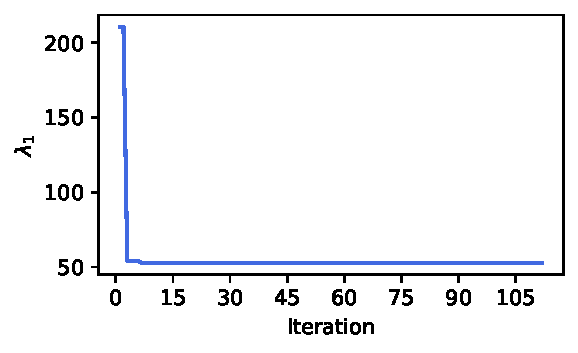
\includegraphics[width = 48mm]{figures/polynomial_4_minimisation_values.pdf}
        \caption{Konvergencija predviđene vrijednosti}
        \label{fig:polynomial_4_minimisation_values}
    \end{subfigure}
    \begin{subfigure}{52mm}
        \centering
        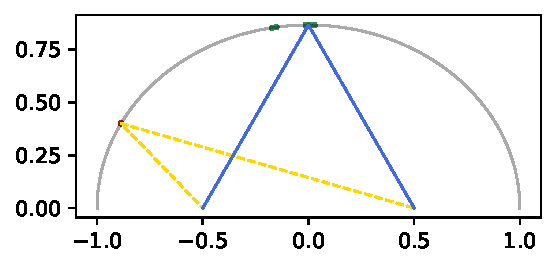
\includegraphics[width = 47mm]{figures/polynomial_4_minimisation_vertices.pdf}
        \caption{Konvergencija vrha}
        \label{fig:polynomial_4_minimisation_vertices}
    \end{subfigure}
    \caption[Minimizacija najmanje svojstvene vrijednosti Laplaceovog operatora polinomom stupnja \ensuremath{\numprint{4}}]{Minimizacija najmanje svojstvene vrijednosti Laplaceovog operatora polinomom stupnja \ensuremath{\numprint{4}}. Na slici~\ref{fig:polynomial_4_minimisation_vertices} vrhovi su obojani s obzirom na predviđenu vrijednost: u crvenim vrhovima je predviđena viša, a u zelinima niža vrijednost. Inicijalni trokut označen je iscrtkanom žutom linijom dok je rezultantni trokut označen punom plavom linijom.}
    \label{fig:polynomial_4_minimisation}
\end{figure}

\par

\begin{figure}[htb!]
    \centering
    \begin{subfigure}{53mm}
        \centering
        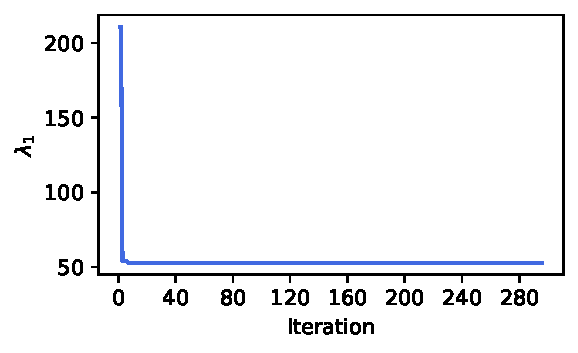
\includegraphics[width = 48mm]{figures/polynomial_5_minimisation_values.pdf}
        \caption{Konvergencija predviđene vrijednosti}
        \label{fig:polynomial_5_minimisation_values}
    \end{subfigure}
    \begin{subfigure}{52mm}
        \centering
        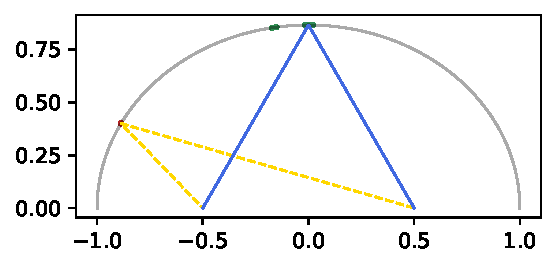
\includegraphics[width = 47mm]{figures/polynomial_5_minimisation_vertices.pdf}
        \caption{Konvergencija vrha}
        \label{fig:polynomial_5_minimisation_vertices}
    \end{subfigure}
    \caption[Minimizacija najmanje svojstvene vrijednosti Laplaceovog operatora polinomom stupnja \ensuremath{\numprint{5}}]{Minimizacija najmanje svojstvene vrijednosti Laplaceovog operatora polinomom stupnja \ensuremath{\numprint{5}}. Na slici~\ref{fig:polynomial_5_minimisation_vertices} vrhovi su obojani s obzirom na predviđenu vrijednost: u crvenim vrhovima je predviđena viša, a u zelinima niža vrijednost. Inicijalni trokut označen je iscrtkanom žutom linijom dok je rezultantni trokut označen punom plavom linijom.}
    \label{fig:polynomial_5_minimisation}
\end{figure}

\par%
\clearpage%
\newpage

\begin{figure}[htb!]
    \centering
    \begin{subfigure}{53mm}
        \centering
        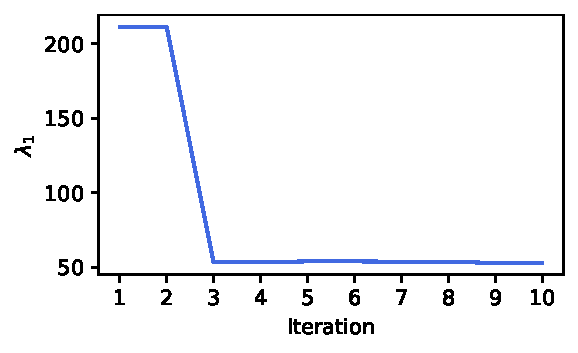
\includegraphics[width = 48mm]{figures/neural_network_minimisation_values.pdf}
        \caption{Konvergencija predviđene vrijednosti}
        \label{fig:neural_network_minimisation_values}
    \end{subfigure}
    \begin{subfigure}{52mm}
        \centering
        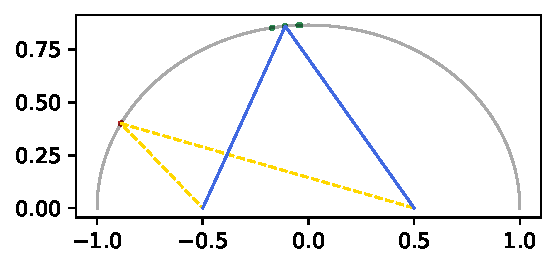
\includegraphics[width = 47mm]{figures/neural_network_minimisation_vertices.pdf}
        \caption{Konvergencija vrha}
        \label{fig:neural_network_minimisation_vertices}
    \end{subfigure}
    \caption[Minimizacija najmanje svojstvene vrijednosti Laplaceovog operatora neuronskom mrežom]{Minimizacija najmanje svojstvene vrijednosti Laplaceovog operatora neuronskom mrežom. Na slici~\ref{fig:neural_network_minimisation_vertices} vrhovi su obojani s obzirom na predviđenu vrijednost: u crvenim vrhovima je predviđena viša, a u zelinima niža vrijednost. Inicijalni trokut označen je iscrtkanom žutom linijom dok je rezultantni trokut označen punom plavom linijom.}
    \label{fig:neural_network_minimisation}
\end{figure}

\par

\begin{figure}[htb!]
    \centering
    \begin{subfigure}{53mm}
        \centering
        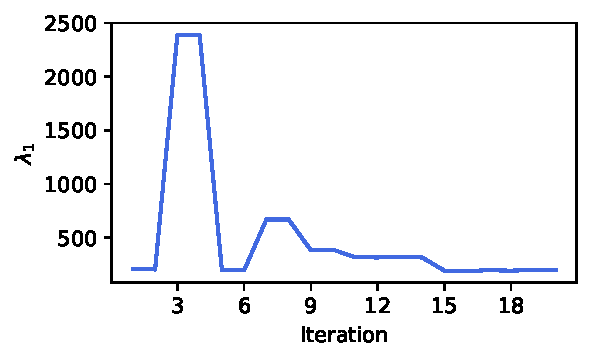
\includegraphics[width = 48mm]{figures/convolutional_neural_network_minimisation_values.pdf}
        \caption{Konvergencija predviđene vrijednosti}
        \label{fig:convolutional_neural_network_minimisation_values}
    \end{subfigure}
    \begin{subfigure}{52mm}
        \centering
        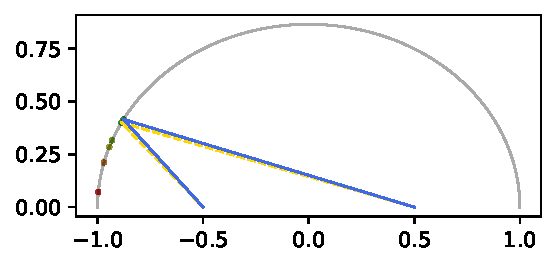
\includegraphics[width = 47mm]{figures/convolutional_neural_network_minimisation_vertices.pdf}
        \caption{Konvergencija vrha}
        \label{fig:convolutional_neural_network_minimisation_vertices}
    \end{subfigure}
    \caption[Minimizacija najmanje svojstvene vrijednosti Laplaceovog operatora konvolucijskom neuronskom mrežom]{Minimizacija najmanje svojstvene vrijednosti Laplaceovog operatora konvolucijskom neuronskom mrežom. Na slici~\ref{fig:convolutional_neural_network_minimisation_vertices} vrhovi su obojani s obzirom na predviđenu vrijednost: u crvenim vrhovima je predviđena viša, a u zelinima niža vrijednost. Inicijalni trokut označen je iscrtkanom žutom linijom dok je rezultantni trokut označen punom plavom linijom.}
    \label{fig:convolutional_neural_network_minimisation}
\end{figure}

\par

Pojava da polinomni modeli uspijevaju minimizirati najmanju svojstvenu vrijednost Laplaceovog operatora mogla se pretpostaviti s obzirom na to da su vrlo uspješni u predviđanju niskih vrijednosti (\seetxt~tablice~\ref{tab:models_rmse} i \ref{tab:models_mape}). Autor ovog rada, doduše, nije uspio objasniti zašto modeli neuronske mreže i konvolucijske neuronske mreže nisu pouzdani modeli u proučavanim problemima minimizacije. Štoviše, ostalo je neobjašnjeno zašto se minimizacija tim modelima izvršava u osjetno manjem broju iteracija, pri čemu neuronska mreža nerijetko izvrši svega $ \numprint{4} $ -- $ \numprint{6} $ iteracija nakon čega se postiže \emph{prividna konvergencija} i minimizacija završava.

\par
